\chapter{Background} \label{sec:background}

\glspl{ann} have shown great improvements over the last years due to increasing compute power, more sophisticated models and smarter training algorithms \todo{cite papers}. \gls{ml} and \glspl{ann} have long found their way into many commercial applications and many scientific fields have successfully applied this relatively new method of data processing to further their own research. \todo{cite papers} It was only logical that researchers and companies have also started to look into the possible benefits this emerging technology could have for Network Security applications \todo{cite papers}. \glspl{ann} are especially suited for \glspl{ids} due to their capability to classify data with high accuracy. To harness the power of \gls{ml} for the purpose of Network Security, we made use of existing methods and models which we will summarize in this section.

\subsection{Machine Learning} \label{sec:background:ml}

\subsection{Artificial Neural Networks} \label{sec:background:ann}

Named after their resemblance to neurons in a brain, \glspl{ann} are systems comprised of connected nodes called \textit{artificial neurons}. Analogous to synapses, nodes communicate \textit{via} connections called \textit{edges} by sending "signals" to other nodes. Signals are represented as scalar real numbers. The output signal from a sending node is multiplied by the weight of the edge the signal is "traveling" on. Each node calculates its output signal by applying a non-linear function to the sum of its input signals. Signals travel forward through the network from the first to the last layer, but usually not within layers. There are various types of \glspl{ann} like \glspl{rnn} or \glspl{cnn} which have many derivations themselves but they all operate on the before stated principal of signals traveling through the network which get transformed at each node by a differentiable non-linear function. The most popular non-linear function at this time is the \gls{relu} function. Without training an \gls{ann} performs an input transformation that depends on the initialization values of its weights, often called \textit{parameters}. The network is trained to perform a desired transformation by adjusting its weights/parameters through virtue of \textit{back-propagation}. The network produces output $\hat{y}$ at the last layer after processing input $x$. A scalar cost/loss value is calculated by a \textit{loss function} $C(\hat{y}, y)$ as a measure of difference between the networks output $\hat{y}$ and the target output $y$. For classification tasks the loss function is usually cross entropy loss \todo{reference cross entropy loss} and for regression \gls{sel} is typically used. Back-propagation computes the gradient of every weight in the network with respect to the loss function by applying the chain-rule for every layer down to every weight. After calculating the gradient for every weight, a gradient method like \gls{sgd} is used to iteratively update all weights in order to minimize $C(\hat{y}, y)$. \todo{find/create graphic}

\subsection{Recurrent Neural Networks} \label{sec:background:rnn}

The broader concept behind all \glspl{rnn} is a cyclic connection which enables the \gls{rnn} to update its state based on past states and current input data \cite{rnn_review}. Typically, an \gls{rnn} consists of standard tanh nodes with corresponding weights. There are different kinds of \glspl{rnn} like continuous-time and discrete-time or finite impulse and infinite impulse \glspl{rnn}. Here we will only look at discrete-time, finite impulse \glspl{rnn} as we will only be using those. This type of network, e.g. the Elman network \cite{rnn_elman}, is capable of processing sequences of variable length by compressing the information from the whole sequence into the \textit{hidden layer}. \todo{give a more formal description of RNNs} The model produces one output token for each input token, so the transformation is sequence-to-sequence where input and output sequences are of equal length. One input sequence consists of a sequence of real valued vectors $x^{(t)} = x^{(1)}, x^{(2)}, ... , x^{(T)}$ where $T$ is the sequence length. From this input sequence, an output sequence of real valued vectors $\hat{y}^{(t)} = \hat{y}^{(1)}, \hat{y}^{(2)}, ... , \hat{y}^{(T)}$ is produced. To train an \gls{rnn} 
pairs of input and target sequences $(x^{(t)}, y^{(t)})$ are provided from which, analogous to the training of \glspl{ann} in general\ref{sec:background:ann}, a differentiable loss function $C(\hat{y}^{(t)}, y^{(t)})$ can be calculated which can again be minimized by applying back-propagation. In theory, \glspl{rnn} can process data sequences of arbitrary length, but the longer the sequence, the deeper the network gets i.e. the longer the gradient paths. This leads to complications when relevant tokens are further apart in the sequence as the \gls{rnn} is not capable of handling such "long-term dependencies" \cite{rnn_review}. Long gradient paths in \glspl{rnn} might also cause the gradient to become either very small or very large, which results in the known \textit{vanishing gradient} or \textit{exploding gradient} problems correspondingly and cause training to either stagnate or diverge. The \gls{lstm} improves upon \glspl{rnn} by making the gradient more stable and allowing long-term dependencies to be considered in the learning process.
\todo{find/create graphic}

\subsection{Long Short-Term Memory}

Introduced by Hochreiter and Schmidhuber in 1997 \cite{lstm_origin}, the \gls{lstm} model mitigates the vanishing and exploding gradient problem by replacing the tanh nodes in the hidden layer of a conventional \gls{rnn} with \textit{memory cells} as seen in \ref{fig:background:lstm}. 
A memory cell is comprised of \textit{input node}, \textit{input gate}, \textit{internal state}, \textit{forget gate} and \textit{output gate}. 

\begin{figure}[h]
	\centering
	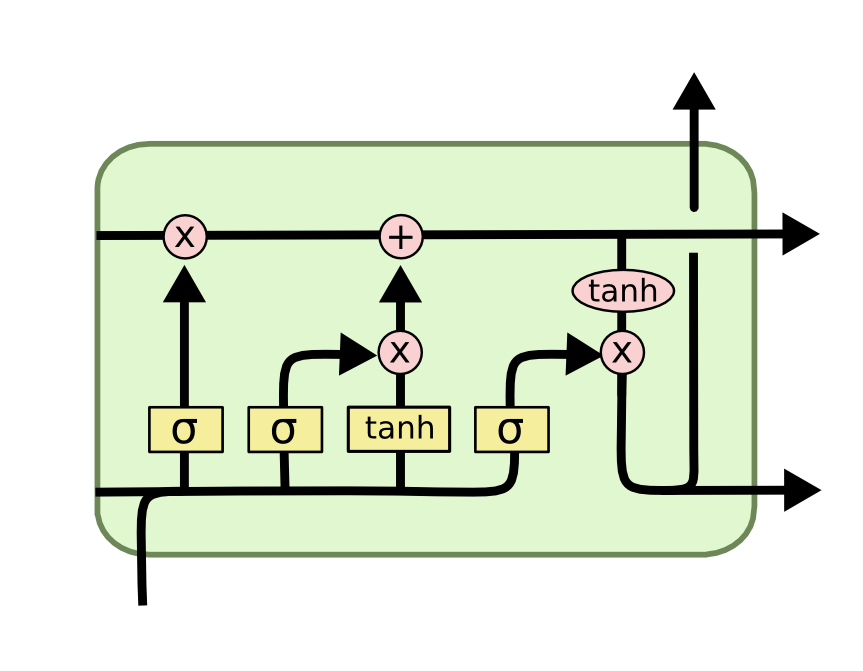
\includegraphics[width=1\textwidth]{img/lstm2.png}
	\caption{One \gls{lstm} memory cell \cite{rnn_zachary}}
	\label{fig:background:lstm}
\end{figure}
In contrast to an ordinary \gls{rnn}, an \gls{lstm} has two memory states: the hidden state $h^{(t)}$ and the \textit{cell state} $C^{(t)}$. Three gates enable the cell to control the flow of information and its effects on the cell state. For this purpose, gates in an \gls{lstm} consist of a point-wise multiplication with a vector that holds values between 0 and 1. The three sigma activations seen in \ref{fig:background:lstm} produce the gate vectors. The input gate $i^{(t)} = \sigma(W^i[h^{(t-1)},x^{(t)}] + b^i)$ controls whether the memory cell is updated. The forget gate $f^{(t)} = \sigma(W^f[h^{(t-1)},x^{(t)}] + b^f)$ controls how much of the old state is to be forgotten. The output gate $o^{(t)} = \sigma(W^o[h^{(t-1)},x^{(t)}] + b^o)$ controls whether the current cell state is made visible. The weight matrices $W^i, W^j$ and $W^o$ decide how information is processed by the cell and are learned parameters. The cell state is updated by addition with the vector $\bar{C}=\tanh(W^C[h^{(t-1)},x^{t}]+b^C)$ after multiplication with the input gate vector $i^{(t)}$. The repeated addition of a tanh activation distributes gradients and vanishing/exploding gradients are mitigated.

\subsection{Adam Optimizer}

\subsection{Attention and Transformers}

2017 Vaswani et al. published a paper with the ominous title "Attention is All you Need" \cite{attention_origin}, referring to the already known attention mechanism which is used to model dependencies within a data sequence over longer distances. The authors proposed the Transformer model consisting entirely of self attention mechanisms to model sequences and therefore diverge from the recurrent architectures of \glspl{rnn} and \glspl{lstm}. Attention is a mechanism to capture contextual relations between tokens in a sequence, e.g. words in a sentence. For every token in the input sequence, an attention vector is generated which represents how relevant other tokens in the input sequence are to the token in question. While attention can be implemented in different ways, the authors chose the scaled dot-product attention defined as 

\begin{equation}
	Attention(Q,K,V) = softmax(\frac{QK^T}{\sqrt{d_k}})V
\end{equation}

\begin{figure}[h]
	\centering
	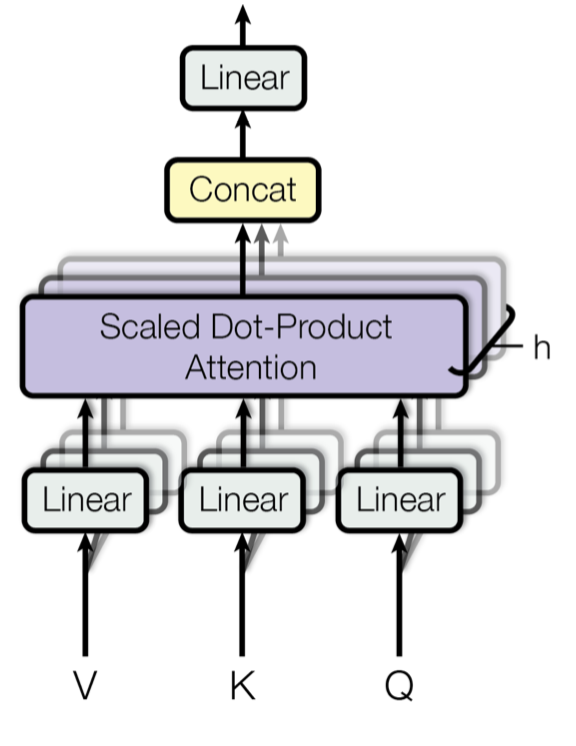
\includegraphics[width=0.3\textwidth]{img/attention.png}
	\caption{Self attention layer of Transformer by \cite{attention_origin}}
	\label{fig:attention}
\end{figure}

"An attention function can be described as mapping a query and a set of key-value pairs to an output" \cite{attention_origin}. $Q$, $K$ and $V$ are matrices composed of query, key and value vectors for every token with respect to every other token in the sequence.
Vaswani et al. proposed the use of Multi-Head Attention mechanism suggesting the use of multiple independent attention heads which are generated by linear projection of the original $Q, K$ and $V$ matrices by different learned matrices $W^Q_i, W^K_i$ and $W^V_i$ for $i = 1, ... ,h$ where $h$ is the number of desired attention heads. The attention vectors of the different attention heads are again concatenated and projected by matrix $W^Z$ again resulting in a single combined attention vector instead of $h$ vectors. This results in the formulation 

\begin{equation}
	head_i = Attention(QW^Q_i, KW^K_i, VW^V_i), i = 1, ..., h
\end{equation}

\begin{equation}
	MultiHead(Q,K,V) = Concat(head_1, ..., head_h)W^O
\end{equation}


\begin{figure}[h]
	\centering
	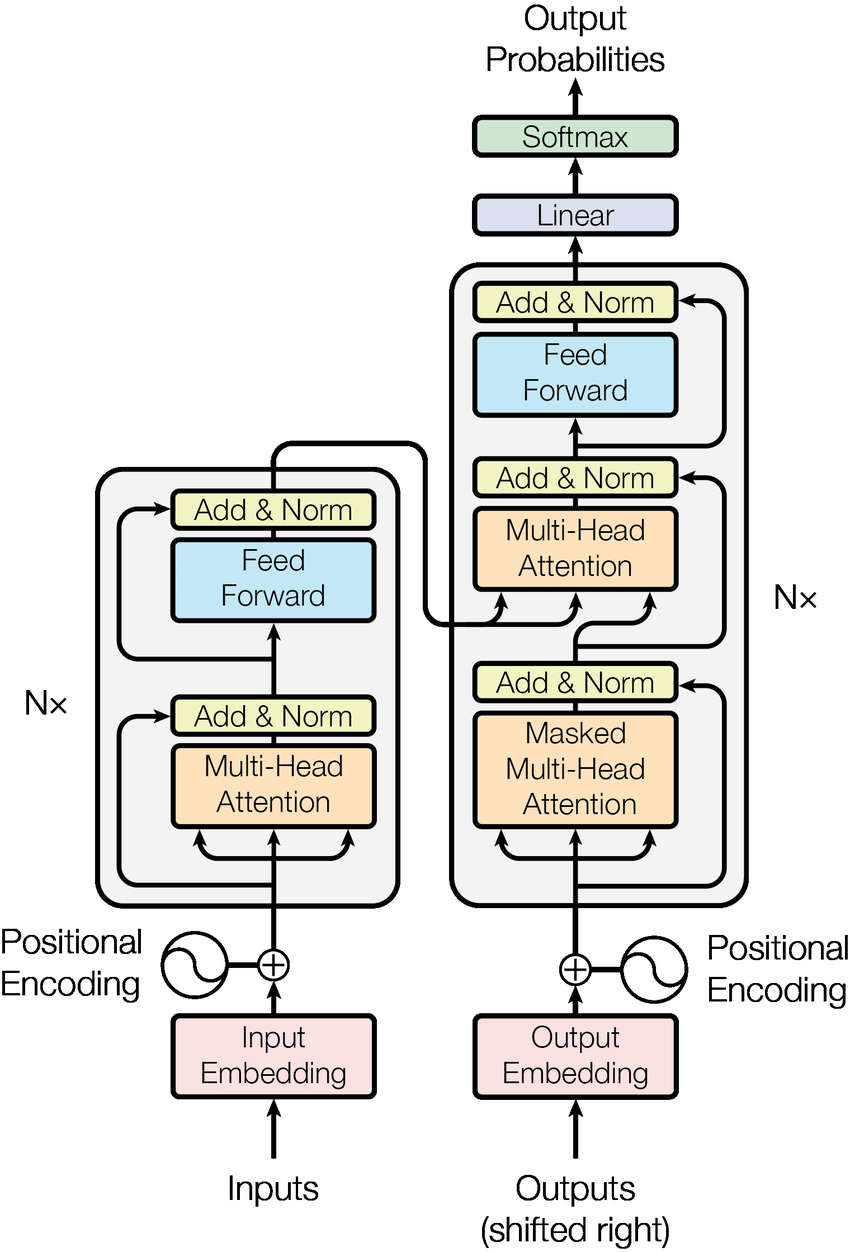
\includegraphics[width=0.7\textwidth]{img/transformer.png}
	\caption{Complete Transformer Encoder-Decoder Model as proposed by \cite{attention_origin}}
	\label{fig:transformer}
\end{figure}

\subsection{Self-supervised Learning}

\subsection{Auto Encoder}

\subsection{Pre-Training and Fine Tuning}

\subsection{Terminology} \label{subsec.terminology}

In addition: Abbreviations and mathematical notation should be put in a list in the beginning of the thesis 

\newpage